\documentclass[lettersize,journal]{IEEEtran}
\usepackage[T1]{fontenc}
\usepackage{newtxtext,newtxmath}   % Times text + math with real bold/italic (IEEE font)
\usepackage{amsmath}
\usepackage{algorithmic}
\usepackage{algorithm}
\usepackage{array}
\usepackage[caption=false,font=normalsize,labelfont=sf,textfont=sf]{subfig}
\usepackage{textcomp}
\usepackage{stfloats}
\usepackage{url}
\usepackage{verbatim}
\usepackage{graphicx}
\usepackage{cite}
\usepackage{booktabs}
\usepackage{xcolor}
\usepackage{tikz}
\usetikzlibrary{arrows.meta,positioning,calc}
\hyphenation{op-tical net-works semi-conduc-tor IEEE-Xplore Embedding-Gemma}

\newcommand{\nQuestions}{64,535}
\newcommand{\nCells}{65}
\newcommand{\nQuestionsRun}{64,478}
\newcommand{\gpuHours}{71}
\newcommand{\nCompared}{29}
\newcommand{\nWithinFive}{12}
\newcommand{\nWithinTen}{20}
\newcommand{\medianAbsDelta}{6.0}
\newcommand{\llamaSCemptyOneK}{25.2}
\newcommand{\llamaSCrtwZero}{205}
\newcommand{\llamaSCwtrZero}{51}
\newcommand{\llamaSCfirstZero}{94.4}
\newcommand{\mistralSCrtwZero}{188}
\newcommand{\mistralSCwtrZero}{29}
\newcommand{\mistralSCfirstZero}{95.6}
\newcommand{\posAccAthree}{60}
\newcommand{\posAccDthree}{43}
\newcommand{\posAccAlong}{42}
\newcommand{\posAccDlong}{23}
\newcommand{\posPickDthree}{14}
\newcommand{\posPickDlong}{8}
\newcommand{\llamaRagRefusalAll}{19.1}

\newcommand{\pRows}{12,950}
\newcommand{\pPos}{3,143}
\newcommand{\pNeg}{9,807}
\newcommand{\pGold}{3,580}
\newcommand{\pPseudo}{9,188}
\newcommand{\pAudited}{182}
\newcommand{\pDupDropped}{1,553}
\newcommand{\pPrefevalTurns}{8,757}
\newcommand{\pOasstPool}{15,427}
\newcommand{\pOasstRev}{fdf72ae0}
\newcommand{\pPersonaFound}{998}
\newcommand{\pOverlapAgree}{95.3}
\newcommand{\pOasstYes}{289}
\newcommand{\pStrictConfirmed}{115}
\newcommand{\pStrictRejected}{174}
\newcommand{\pGenericExcl}{1,384}
\newcommand{\pStrictExcl}{791}
\newcommand{\pGenericPrec}{0.28}
\newcommand{\pStrictPrec}{0.60}
\newcommand{\pAuditBefore}{73.9}
\newcommand{\pAuditAfter}{90.7}
\newcommand{\pKappa}{0.48}
\newcommand{\pTopicRateLo}{0.35}
\newcommand{\pTopicRateHi}{0.41}
\newcommand{\pFOneLo}{0.969}
\newcommand{\pFOneHi}{0.976}
\newcommand{\pBestEnsFOne}{0.977}
\newcommand{\pBestEnsMembers}{TinyLlama + Qwen3}
\newcommand{\pErrCorrLo}{0.68}
\newcommand{\pErrCorrHi}{0.75}
\newcommand{\pDisagreeMax}{0.9}
\newcommand{\pLlmFOne}{0.879}
\newcommand{\pLlmPrec}{0.787}
\newcommand{\pLlmRec}{0.996}
\newcommand{\pLlmFpr}{16.5}
\newcommand{\pLlmLat}{72}
\newcommand{\pDistilLat}{1.4}
\newcommand{\pSpeedup}{51}
\newcommand{\pDistilSameFOne}{0.990}
\newcommand{\pOodLo}{0.1}
\newcommand{\pOodHi}{1.5}
\newcommand{\pTotalTrainH}{4.3}
\newcommand{\pOasstRecLo}{16}
\newcommand{\pOasstRecHi}{26}
\newcommand{\pOasstPosTest}{114}

\newcommand{\qSimExR}{40.0}
\newcommand{\qGemExR}{82.7}
\newcommand{\qSimImR}{58.5}
\newcommand{\qGemImR}{87.7}
\newcommand{\qSimExROne}{8.5}
\newcommand{\qGemExROne}{82.4}
\newcommand{\qGemLat}{15.6}
\newcommand{\qMxbaiExR}{77.9}
\newcommand{\qEFiveExR}{30.7}
\newcommand{\qReplyGap}{0.6}
\newcommand{\qMemEx}{98.6}
\newcommand{\qMemIm}{99.9}
\newcommand{\qFalseSixteen}{0.22}
\newcommand{\qFalseTwentyThree}{0.65}
\newcommand{\qMissedEx}{14}
\newcommand{\qLlExMemThree}{96.5}
\newcommand{\qLlExRagThree}{74.8}
\newcommand{\qLlImMemThree}{83.5}
\newcommand{\qLlImRagThree}{73.7}
\newcommand{\qLlExGemThree}{93.9}
\newcommand{\qMiMemTwentyThree}{88.6}
\newcommand{\qMiRagTwentyThree}{53.7}
\newcommand{\qMiRemTwentyThree}{46.9}
\newcommand{\qMiZsTwentyThree}{37.6}
\newcommand{\qMiMemTen}{93.7}
\newcommand{\qMiGainTwentyThree}{34.9}
\newcommand{\qMiImMemZero}{81.9}
\newcommand{\qMiImRemZero}{88.4}
\newcommand{\qMiImMemThree}{79.8}
\newcommand{\qMiImRagThree}{64.0}
\newcommand{\qLostEx}{49}
\newcommand{\qLostExParse}{40}
\newcommand{\qLostIm}{99}
\newcommand{\qLostImParse}{65}
\newcommand{\qLostImGold}{98}
\newcommand{\qMiCondTen}{94.5}
\newcommand{\qMiCondTwentyThree}{89.1}
\newcommand{\qMiMissAccLo}{36}
\newcommand{\qMiMissAccHi}{50}
\newcommand{\qStExAll}{90.5}
\newcommand{\qStExTop}{93.9}
\newcommand{\qStImAll}{71.1}
\newcommand{\qStImTop}{77.0}
\newcommand{\qStKeepEx}{97.4}
\newcommand{\qStKeepIm}{98.5}
\newcommand{\qTokZs}{3,282}
\newcommand{\qTokMem}{3,343}
\newcommand{\qTokAdd}{61}
\newcommand{\qClfLat}{1.4}
\newcommand{\qTotalQ}{46,000}
\newcommand{\qGpuHours}{44}

\graphicspath{{figures/}}
\definecolor{boxblue}{HTML}{E8F1FC}
\definecolor{boxline}{HTML}{2A78D6}
\definecolor{boxgreen}{HTML}{E7F6EF}
\definecolor{linegreen}{HTML}{1BAF7A}
\definecolor{boxorange}{HTML}{FDEEE7}
\definecolor{lineorange}{HTML}{EB6834}

\begin{document}

\title{Improving Long-Context Preference Following in LLMs via a Trained Preference-Detection Classifier and Enhanced Retrieval}

\author{Krishna Jhanwar - 12341250}

\maketitle

\begin{abstract}
Large language models (LLMs) used as assistants are expected to remember what a user has told them, yet PrefEval (ICLR 2025) shows
that their preference following collapses as unrelated conversation accumulates. This project addresses two weaknesses that the paper
identifies: an outdated retriever and the absence of any persistent preference state. First, I rebuilt PrefEval's classification
benchmark to run fully locally and reproduced its five baselines with two of the paper's models (Llama-3-8B, Mistral-7B-v0.2;
\nQuestions{} questions). Second, I trained a small classifier that detects preference-stating user turns (DistilBERT, F1~0.969 on unseen
topics, 1.4\,ms per message). Third, the classifier feeds a structured \emph{preference memory} that is restated before each question,
and a modern encoder (EmbeddingGemma-2) replaces the paper's 2021 SimCSE retriever. On the same questions, prompts and metric as the baselines,
the memory beats every baseline at every context length from 1k tokens up, for both models and both preference forms. It reaches
\qMiMemTwentyThree\% at 23k tokens with Mistral, versus \qMiRagTwentyThree\% for the paper's best method (RAG). Ablations show that the new encoder
alone fixes the retrieval bottleneck for explicit preferences, that adding retrieved raw messages on top of memory does not help, and that
retrieving \emph{over} the memory keeps accuracy stable when the memory holds many preferences.
\end{abstract}

\begin{IEEEkeywords}
Personalization, preference following, long context, retrieval-augmented generation, conversational memory, text classification.
\end{IEEEkeywords}

%===============================================================================
\section{Introduction}
\IEEEPARstart{A}{n} assistant that is told \emph{``I avoid gluten because of a severe intolerance''} and later recommends a bakery has
failed the user. PrefEval~\cite{prefeval} measures exactly this. A preference is stated at the start of a conversation, unrelated
multi-session chat follows, and a later question can only be answered well if the preference is remembered. Even strong models degrade
quickly, and the paper's best mitigation, retrieval-augmented generation (RAG) with a SimCSE~\cite{simcse} encoder, also loses accuracy as the
conversation grows.

\textbf{Project criterion.} PrefEval's code is public, so this project follows the criterion \emph{``code available: address its
limitations and propose a solution''}. It first reproduces the baselines locally, then proposes and evaluates an improvement.

\textbf{Team and contributions.} This is an individual project. Krishna Jhanwar (12341250, \texttt{krishnaj@iitbhilai.ac.in}) is
responsible for all parts: problem definition and proposal, design decisions, data audit, running all experiments, analysis and reports.
Tools and major prompts used are listed in the Appendix.

\textbf{Problem statement and scope.} The goal is to improve preference following in long conversations for open 7--8B models running on a
single consumer GPU. The scope is PrefEval's \emph{classification} (multiple-choice) task, for explicit and implicit choice-based preferences, at
the paper's context lengths of 0.2k--23k tokens. The generation task is out of scope because its judge (Claude-3-Sonnet via Bedrock) is not
reproducible locally. The problem matters for ML because it isolates two open issues in deployed LLMs: using information far back in a long
context~\cite{lostmiddle}, and maintaining user state over many sessions.

\textbf{Contributions.}
(1)~A fully local, verified reproduction of PrefEval's classification baselines (\nQuestions{} questions, two models, five methods).
(2)~A preference-detection classifier, trained with topic-held-out cross-validation and audited pseudo-labels, that is 51$\times$ faster and more
accurate than prompting an 8B LLM.
(3)~A retrieval benchmark of five current encoders against the paper's retriever.
(4)~A classifier-driven preference memory, evaluated against all baselines on \qTotalQ{} further questions, with ablations and a
multi-preference stress test.

%===============================================================================
\section{Related Work}
\textbf{Preference following.} PrefEval~\cite{prefeval} evaluates explicit and implicit preferences over long multi-session contexts and
compares zero-shot, reminder, self-critic, few-shot chain-of-thought and RAG prompting.
\textbf{Long context.} Models use information at the start of long inputs poorly~\cite{lostmiddle}; PrefEval places the preference exactly there.
\textbf{Retrieval.} RAG adds retrieved text to the prompt. PrefEval uses SimCSE~\cite{simcse}; since then, retrieval-trained encoders
such as BGE~\cite{bge}, E5~\cite{e5}, mxbai-embed-large~\cite{mxbai} and EmbeddingGemma~\cite{embeddinggemma} have become standard.
\textbf{Memory.} Systems such as MemGPT~\cite{memgpt} let an LLM write and read long-term memory, which costs extra LLM calls.
This project instead uses a small \emph{trained} classifier to decide what is stored, which needs one cheap forward pass per turn.

%===============================================================================
\section{Proposed Methodology}
The work has three phases; each builds on the previous one (Fig.~\ref{fig:pipeline}).

\begin{figure*}[!t]
\centering
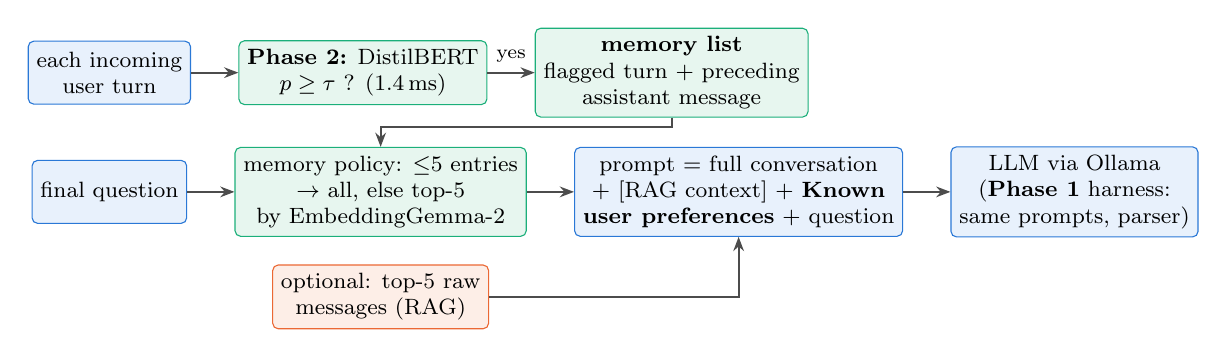
\begin{tikzpicture}[font=\footnotesize, node distance=3.5mm and 6mm,
  box/.style={draw=boxline, fill=boxblue, rounded corners=2pt, align=center, inner sep=3pt, minimum height=8mm},
  gbox/.style={draw=linegreen, fill=boxgreen, rounded corners=2pt, align=center, inner sep=3pt, minimum height=8mm},
  obox/.style={draw=lineorange, fill=boxorange, rounded corners=2pt, align=center, inner sep=3pt, minimum height=8mm},
  arr/.style={-{Stealth[length=1.8mm]}, thick, draw=black!70}]
\node[box] (turn) {each incoming\\user turn};
\node[gbox, right=of turn] (clf) {\textbf{Phase 2:} DistilBERT\\$p \geq \tau$ ? (1.4\,ms)};
\node[gbox, right=of clf] (mem) {\textbf{memory list}\\flagged turn + preceding\\assistant message};
\node[box, below=7mm of turn] (q) {final question};
\node[gbox, right=of q] (sel) {memory policy: $\leq$5 entries\\$\rightarrow$ all, else top-5\\by EmbeddingGemma-2};
\node[obox, below=of sel] (rag) {optional: top-5 raw\\messages (RAG)};
\node[box, right=of sel] (prompt) {prompt = full conversation\\+ [RAG context] + \textbf{Known}\\\textbf{user preferences} + question};
\node[box, right=of prompt] (llm) {LLM via Ollama\\(\textbf{Phase 1} harness:\\same prompts, parser)};
\draw[arr] (turn) -- (clf);
\draw[arr] (clf) -- node[above, font=\scriptsize]{yes} (mem);
\draw[arr] (mem.south) |- ($(sel.north)+(0,2.5mm)$) -- (sel.north);
\draw[arr] (q) -- (sel);
\draw[arr] (sel) -- (prompt);
\draw[arr] (rag.east) -| (prompt.south);
\draw[arr] (prompt) -- (llm);
\end{tikzpicture}
\caption{Proposed pipeline. Phase~1 provides the local evaluation harness and baselines, Phase~2 the classifier, Phase~3 the memory,
the memory policy and the retriever (green: new components; orange: retrieval over raw messages, evaluated as an ablation).}
\label{fig:pipeline}
\end{figure*}

\subsection{Phase 1: local reproduction of the baselines}
PrefEval's released code calls Amazon Bedrock for every model, and an earlier local attempt failed with several unrelated errors. I rebuilt
the classification pipeline around the \emph{original} prompt-building functions (vendored unchanged from the upstream repository) and replaced
only the inference call with Ollama in raw-prompt mode. The model therefore sees exactly the text that Bedrock received. Answers are
parsed with the original strict \texttt{<choice>X</choice>} parser. Every question is written to disk as soon as it is answered, so a run
resumes after any interruption. Five issues that would have silently biased the reproduction were found and fixed:
\begin{itemize}
  \item a duplicated start-of-sequence token;
  \item trailing whitespace in the Llama self-critic templates, which made the model stop immediately;
  \item silent prompt truncation at long context;
  \item two defects in the released retrieval data (one truncated file, seven files that end early);
  \item a GPU-memory limit at 32k context, solved with flash attention and an 8-bit KV cache for Mistral, enforced by a per-model settings guard.
\end{itemize}

\subsection{Phase 2: preference-detection classifier}
\emph{Task:} given one user message (text only), decide whether it states a lasting personal preference.
\emph{Data:} \pRows{} messages. \pGold{} labels come from PrefEval's structure (preference sentences and choice selections are positive;
queries and questions negative). \pPseudo{} are pseudo-labels from Llama-3-8B for persona-dialogue turns and 5{,}000 OpenAssistant
messages. A manual audit of 200 pseudo-labels exposed two systematic error types; targeted refinement raised agreement with the human labels from
\pAuditBefore\% to \pAuditAfter\%, and \pAudited{} rows carry the human label.
\emph{Leakage control:} topic-level 5-fold cross-validation (test topics are never seen in training), and the LMSYS distractor turns are never
trained on. \emph{Models:} DistilBERT~\cite{distilbert}, ModernBERT~\cite{modernbert}, and TinyLlama-1.1B~\cite{tinyllama} and
Qwen3-1.7B~\cite{qwen3} with LoRA~\cite{lora}. The decision threshold is tuned on each fold's validation topics.

\subsection{Phase 3: preference memory and modern retrieval}
\textbf{Step 1, retrieval benchmark (no LLM calls).} Five encoders (bge-base/large-v1.5~\cite{bge}, e5-base-v2~\cite{e5},
mxbai-embed-large~\cite{mxbai}, EmbeddingGemma-2~\cite{embeddinggemma}) are compared with the paper's stored SimCSE scores. Each one must find the
preference message among all messages before the question, using each model's official query/document prompts and weights pinned to an
exact version. Because a bi-encoder embeds each message independently, pre-computing embeddings gives exactly what a live system computes turn
by turn; the real-time cost is reported as latency.

\textbf{Step 2, memory.} Each user turn is scored by the Phase~2 classifier. For a question of topic $t$, the fold model that was \emph{tested}
on $t$ is used, so the classifier never saw that topic. A flagged turn is stored together with the assistant message just before it. For
implicit preferences, the entry is therefore the options list plus the user's selection: Step~1 showed that the selection alone (e.g.\ ``I'll take
the second one'') is meaningless without the options. At question time, all entries go into the prompt if there are at most five; otherwise
the five most similar to the question are selected with EmbeddingGemma-2. They are inserted as a short ``Known user preferences'' block
right before the question.

\textbf{Methods compared.} Each new method changes exactly one thing compared with a Phase~1 baseline:
(i) \emph{Memory} = the zero-shot prompt plus the memory block;
(ii) \emph{RAG-Gemma} = the paper's RAG prompt with EmbeddingGemma-2 replacing SimCSE;
(iii) \emph{Memory+RAG} = (ii) plus the memory block.
With SimCSE's retrieved messages substituted, our RAG prompt is byte-identical to the Phase~1 RAG prompt, and the memory prompt with an empty
memory is byte-identical to the zero-shot prompt (checked on 96 prompts). Every accuracy difference is therefore caused by the method itself.

%===============================================================================
\section{Experimental Setup}
\textbf{Dataset.} PrefEval~\cite{prefeval} (public, in the GitHub repository and on HuggingFace): 1{,}000 preference--question pairs over
20 topics in each preference form. Each question has four options, exactly one of which respects the preference. Distractor turns come from
LMSYS-Chat-1M~\cite{lmsys}. The paper's context rows 0.2k/1k/3k/10k/16k/23k tokens correspond to 0/3/8/28/48/68 inserted turn pairs. The
explicit and implicit choice-based forms are used; Phase~2 additionally uses OpenAssistant \texttt{oasst1}.

\textbf{Models.} Llama-3-8B-Instruct~\cite{llama3} (8k context, so 0.2k--3k only) and Mistral-7B-Instruct-v0.2~\cite{mistral} (up to 23k), both used
in the paper, served as 8-bit weights by Ollama with greedy decoding (temperature 0, seed 41). Mixtral-8x7B does not fit the hardware.

\textbf{Metric.} Accuracy with the paper's strict answer parser, macro-averaged over the 20 topics, as in the paper. A lenient parse is logged as a
diagnostic only. The classifier is evaluated with precision, recall and F1 on unseen-topic test folds.

\textbf{Protocol.} Every Phase~3 cell uses the same 1{,}000 questions, option order and prompts as its Phase~1 baseline, so all comparisons are
paired. The paper's RAG has stored scores for 949 explicit and 973 implicit questions; RAG comparisons are additionally reported on exactly those.

\textbf{Resources.} One workstation: NVIDIA RTX~3060 (12\,GB), Intel i7-12700, 15\,GB RAM. Software: Python~3.11, PyTorch, HuggingFace
\texttt{transformers} and \texttt{peft}, sentence-transformers, scikit-learn, Ollama. In total, about 120 GPU-hours: Phase~1 \gpuHours\,h,
Phase~3 \qGpuHours\,h, plus classifier training and pseudo-labelling. All long runs ran in \texttt{tmux} and resume per question.

%===============================================================================
\section{Results and Analysis}

\subsection{Phase 1: reproduction}
Of the \nCompared{} cells with a published number (excluding the trivial 0.2k row), \nWithinFive{} are within 5 points of the paper and
\nWithinTen{} within 10 (median absolute difference \medianAbsDelta{} points; Fig.~\ref{fig:vspaper}, Table~\ref{tab:p1}). The paper's
qualitative findings reproduce:
\begin{itemize}
  \item accuracy collapses with context length (Llama zero-shot: 94.2\% at 0.2k $\rightarrow$ 43.3\% at 3k);
  \item Reminder and RAG are the strongest baselines;
  \item self-critique often overturns correct answers;
  \item implicit preferences are harder.
\end{itemize}
The largest gap, Mistral RAG at long context (53.7\% vs.\ 75\%), coincides with the 8-bit KV cache needed to fit 32k tokens in 12\,GB.
At long context the model also falls back on answer position: Mistral zero-shot is right \posAccAlong\% of the time when the answer is A,
but only \posAccDlong\% when it is D.

\begin{figure*}[!t]
\centering
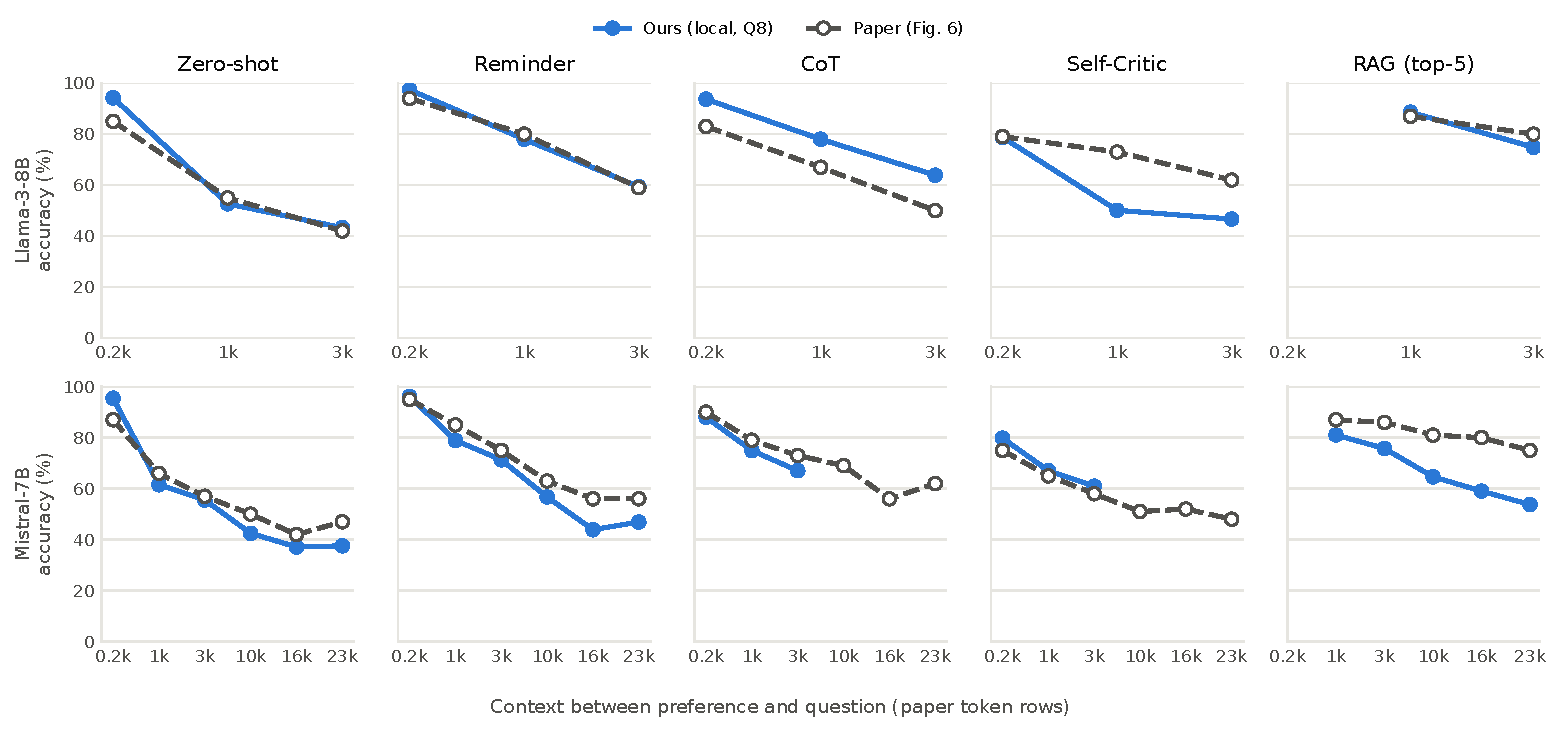
\includegraphics[width=0.82\textwidth]{fig_vs_paper.pdf}
\caption{Phase~1: explicit-preference accuracy, our local reproduction (solid) vs.\ the paper's Figure~6 (dashed).}
\label{fig:vspaper}
\end{figure*}

\begin{table*}[!t]
\caption{Phase 1 reproduction, explicit preference: ours / paper (difference), accuracy \%.}
\label{tab:p1}
\centering\small
\textbf{Llama-3-8B-Instruct}\\[2pt]
\begin{tabular}{lrrr}
\toprule
Method & 0.2k (0) & 1k (3) & 3k (8) \\
\midrule
Zero-shot & 94.2 / 85 (+9.2) & 52.7 / 55 ($-$2.3) & 43.3 / 42 (+1.3) \\
Reminder & 97.4 / 94 (+3.4) & 78.0 / 80 ($-$2.0) & 59.4 / 59 (+0.4) \\
CoT & 93.7 / 83 (+10.7) & 78.0 / 67 (+11.0) & 63.9 / 50 (+13.9) \\
Self-Critic & 78.8 / 79 ($-$0.2) & 50.1 / 73 ($-$22.9) & 46.7 / 62 ($-$15.3) \\
RAG (top-5) & -- & 88.6 / 87 (+1.6) & 74.8 / 80 ($-$5.2) \\
\bottomrule
\end{tabular}
\\[6pt]
\textbf{Mistral-7B-Instruct-v0.2}\\[2pt]
\resizebox{0.95\textwidth}{!}{\begin{tabular}{lrrrrrr}
\toprule
Method & 0.2k (0) & 1k (3) & 3k (8) & 10k (28) & 16k (48) & 23k (68) \\
\midrule
Zero-shot & 95.5 / 87 (+8.5) & 61.5 / 66 ($-$4.5) & 55.5 / 57 ($-$1.5) & 42.5 / 50 ($-$7.5) & 37.1 / 42 ($-$4.9) & 37.6 / 47 ($-$9.4) \\
Reminder & 96.2 / 95 (+1.2) & 78.9 / 85 ($-$6.1) & 71.3 / 75 ($-$3.7) & 56.7 / 63 ($-$6.3) & 43.9 / 56 ($-$12.1) & 46.9 / 56 ($-$9.1) \\
CoT & 88.0 / 90 ($-$2.0) & 74.9 / 79 ($-$4.1) & 67.0 / 73 ($-$6.0) & -- & -- & -- \\
Self-Critic & 79.8 / 75 (+4.8) & 67.0 / 65 (+2.0) & 61.0 / 58 (+3.0) & -- & -- & -- \\
RAG (top-5) & -- & 81.0 / 87 ($-$6.0) & 75.7 / 86 ($-$10.3) & 64.6 / 81 ($-$16.4) & 59.0 / 80 ($-$21.0) & 53.7 / 75 ($-$21.3) \\
\bottomrule
\end{tabular}
}
\end{table*}

\subsection{Phase 2: classifier}
All four classifiers reach F1 \pFOneLo--\pFOneHi{} on unseen topics, and their differences are small (Table~\ref{tab:p2}).
On the same 2{,}000 messages, a zero-shot prompted Llama-3-8B reaches only F1~\pLlmFOne{} and wrongly flags 16.5\% of non-preference messages,
while DistilBERT is \pSpeedup$\times$ faster (\pDistilLat\,ms vs.\ \pLlmLat\,ms per message). On the LMSYS turns that Phase~3 replays, the models
raise false alarms on only \pOodLo--\pOodHi\% of messages. DistilBERT was selected for Phase~3 as the fastest model with a low false-alarm rate.

\begin{table*}[!t]
\caption{Phase 2: preference-detection classifiers, pooled over unseen-topic test folds. OOD flags = false alarms on LMSYS distractor turns.}
\label{tab:p2}
\centering\small
\begin{tabular}{lrrrrrrrrrr}
\toprule
Model & F1 & Prec. & Rec. & F1 std & AUC & ECE & OOD flags & ms/msg & Trainable & Train min \\
\midrule
DistilBERT & 0.969 & 0.983 & 0.955 & 0.007 & 0.994 & 0.008 & 0.4\% & 1.4 & 67M & 14 \\
ModernBERT & 0.972 & 0.988 & 0.956 & 0.004 & 0.995 & 0.009 & 0.2\% & 6.5 & 150M & 32 \\
TinyLlama-1.1B (LoRA) & 0.974 & 0.988 & 0.961 & 0.006 & 0.997 & 0.010 & 0.1\% & 17.1 & 13M & 91 \\
Qwen3-1.7B (LoRA) & 0.976 & 0.988 & 0.965 & 0.006 & 0.997 & 0.009 & 1.5\% & 25.1 & 17M & 120 \\
\bottomrule
\end{tabular}

\end{table*}

\subsection{Phase 3, Step 1: retrieval}
EmbeddingGemma-2 finds the explicit preference in its top~5 for \qGemExR\% of questions at 23k tokens, versus \qSimExR\% for SimCSE
(implicit: \qGemImR\% vs.\ \qSimImR\%; Table~\ref{tab:retrieval}, Fig.~\ref{fig:retrieval}). SimCSE almost never ranks the preference first
(recall@1 \qSimExROne\% at 1k, vs.\ \qGemExROne\%). Newer is not automatically better: e5-base-v2 falls below SimCSE on long explicit
conversations (\qEFiveExR\% at 23k). EmbeddingGemma-2 was chosen (\qGemLat\,ms per message). On implicit preferences, no encoder ranks the user's
selection first (recall@1 5--28\%), which motivated storing it together with the options message. Verifying the benchmark also revealed an
upstream data quirk: in 13 of 20 topics, the file that maps SimCSE scores back to message text is shifted by one exchange. Recall and rank are
unaffected, because they depend only on the scores.

\begin{table*}[!t]
\caption{Phase 3, Step 1: retrieval of the preference message (recall@5 unless noted), on the questions with stored SimCSE scores.}
\label{tab:retrieval}
\centering\small
\begin{tabular}{lr|ccccc|cccc|r}
\toprule
 & & \multicolumn{5}{c|}{Explicit} & \multicolumn{4}{c|}{Implicit-choice} &  \\
Retriever & Params & R@5 1k & 3k & 10k & 23k & R@1 23k & R@5 1k & 3k & 10k & 23k & ms/msg \\
\midrule
SimCSE (paper) & 355M & 0.95 & 0.83 & 0.60 & 0.40 & 0.05 & 0.97 & 0.90 & 0.75 & 0.58 & -- \\
\midrule
bge-base-v1.5 & 110M & 0.96 & 0.92 & 0.68 & 0.57 & 0.29 & 1.00 & 0.99 & 0.95 & 0.92 & 3.5 \\
e5-base-v2 & 110M & 0.96 & 0.86 & 0.44 & 0.31 & 0.12 & 1.00 & 1.00 & 0.96 & 0.93 & 3.6 \\
bge-large-v1.5 & 335M & 0.98 & 0.95 & 0.74 & 0.66 & 0.43 & 1.00 & 0.99 & 0.92 & 0.89 & 9.8 \\
mxbai-embed-large & 335M & 1.00 & 0.99 & 0.83 & 0.78 & 0.53 & 1.00 & 0.98 & 0.91 & 0.88 & 9.8 \\
\textbf{EmbeddingGemma-2} & 744M & 1.00 & 1.00 & 0.90 & 0.83 & 0.53 & 1.00 & 0.99 & 0.92 & 0.88 & 15.6 \\
\bottomrule
\end{tabular}

\end{table*}

\begin{figure}[!t]
\centering
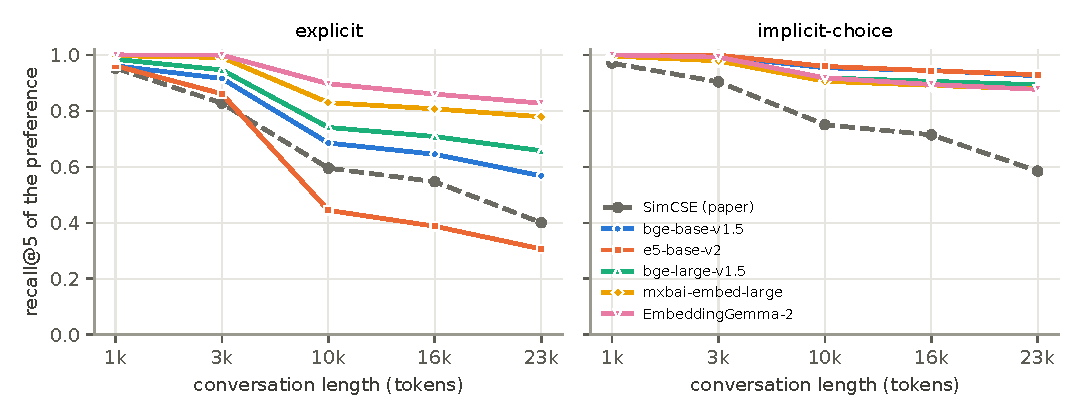
\includegraphics[width=\columnwidth]{p3_retrieval.pdf}
\caption{Recall@5 of the preference message versus conversation length.}
\label{fig:retrieval}
\end{figure}

\subsection{Phase 3, Step 2: memory quality}
The classifier places the true preference in memory for \qMemEx\% of explicit and \qMemIm\% of implicit questions. The \qMissedEx{} explicit
misses are mostly phrased as dislikes, e.g.\ ``I'm uncomfortable with invisible fences''. False entries appear only at 16k (\qFalseSixteen{} per
question) and 23k (\qFalseTwentyThree): two LMSYS messages that read like stated opinions. Memories therefore hold 1--3 entries.

\subsection{Phase 3: main comparison with the baselines}
Tables~\ref{tab:llama}--\ref{tab:mistral} and Fig.~\ref{fig:main} give the end-to-end results.

\begin{table}[!t]
\caption{Llama-3-8B, accuracy \% (macro over 20 topics). Bold: best per column.}
\label{tab:llama}
\centering
\resizebox{\columnwidth}{!}{\begin{tabular}{l|ccc|ccc}
\toprule
 & \multicolumn{3}{c|}{Explicit} & \multicolumn{3}{c}{Implicit-choice} \\
Method & 0.2k & 1k & 3k & 0.2k & 1k & 3k \\
\midrule
Zero-shot & 94.2 & 52.7 & 43.3 & 77.0 & 53.3 & 46.0 \\
Reminder & 97.4 & 78.0 & 59.4 & \textbf{91.0} & 77.0 & 60.3 \\
CoT & 93.7 & 78.0 & 63.9 & 84.4 & 70.3 & 61.7 \\
Self-Critic & 78.8 & 50.1 & 46.7 & 66.1 & 50.1 & 38.7 \\
RAG, SimCSE (paper) & -- & 88.6 & 74.8 & -- & 82.8 & 73.7 \\
\midrule
\textbf{Memory (ours)} & \textbf{97.7} & \textbf{96.0} & \textbf{96.5} & 90.0 & \textbf{86.3} & \textbf{83.5} \\
RAG, EmbeddingGemma-2 (ours) & -- & 94.7 & 93.9 & -- & 83.6 & 79.1 \\
Memory + RAG (ours) & -- & 93.4 & 92.9 & -- & 84.2 & 75.4 \\
\bottomrule
\end{tabular}
}
\end{table}

\begin{table}[!t]
\caption{Mistral-7B-v0.2, accuracy \%. CoT and Self-Critic were not run beyond 3k (as in the paper).}
\label{tab:mistral}
\centering
\resizebox{\columnwidth}{!}{\begin{tabular}{l|cccccc}
\toprule
 & \multicolumn{6}{c}{Explicit} \\
Method & 0.2k & 1k & 3k & 10k & 16k & 23k \\
\midrule
Zero-shot & 95.5 & 61.5 & 55.5 & 42.5 & 37.1 & 37.6 \\
Reminder & 96.2 & 78.9 & 71.3 & 56.7 & 43.9 & 46.9 \\
CoT & 88.0 & 74.9 & 67.0 & -- & -- & -- \\
Self-Critic & 79.8 & 67.0 & 61.0 & -- & -- & -- \\
RAG, SimCSE (paper) & -- & 81.0 & 75.7 & 64.6 & 59.0 & 53.7 \\
\midrule
\textbf{Memory (ours)} & \textbf{97.1} & \textbf{94.7} & \textbf{94.9} & 93.7 & \textbf{92.4} & \textbf{88.6} \\
RAG, EmbeddingGemma-2 (ours) & -- & 85.3 & 86.1 & -- & -- & -- \\
Memory + RAG (ours) & -- & 94.2 & 94.4 & \textbf{94.1} & 90.6 & 87.5 \\
\bottomrule
\end{tabular}
}\\[4pt]
\resizebox{0.62\columnwidth}{!}{\begin{tabular}{l|ccc}
\toprule
 & \multicolumn{3}{c}{Implicit-choice} \\
Method & 0.2k & 1k & 3k \\
\midrule
Zero-shot & 81.0 & 50.8 & 47.5 \\
Reminder & \textbf{88.4} & 71.9 & 63.1 \\
CoT & 74.0 & 60.2 & 59.5 \\
Self-Critic & 67.2 & 51.8 & 50.9 \\
RAG, SimCSE (paper) & -- & 69.0 & 64.0 \\
\midrule
\textbf{Memory (ours)} & 81.9 & \textbf{81.4} & \textbf{79.8} \\
RAG, EmbeddingGemma-2 (ours) & -- & 67.2 & 65.0 \\
Memory + RAG (ours) & -- & 79.3 & 78.3 \\
\bottomrule
\end{tabular}
}
\end{table}

\begin{figure*}[!t]
\centering
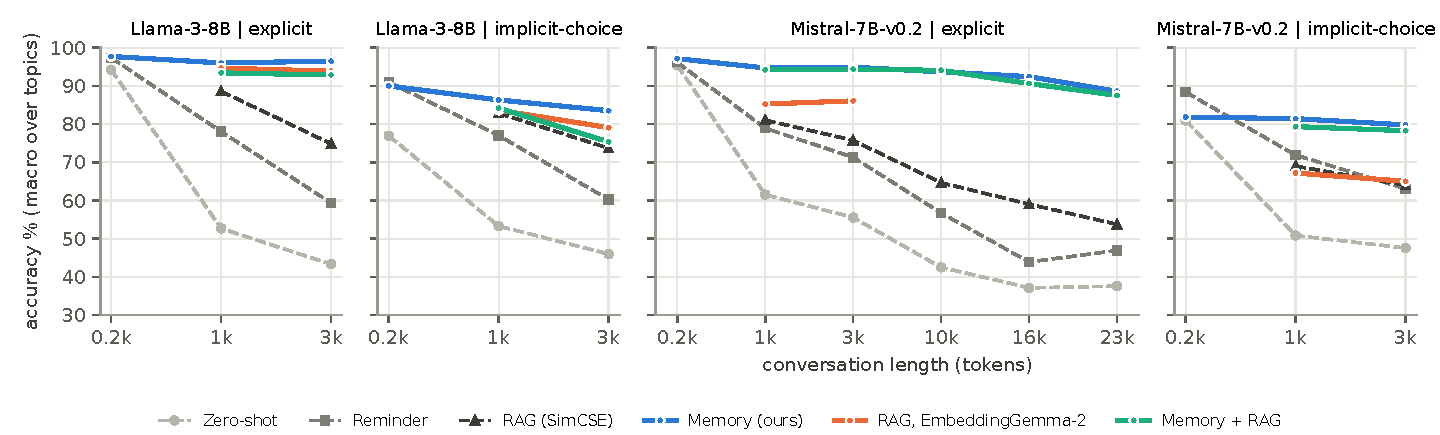
\includegraphics[width=\textwidth]{p3_main.pdf}
\caption{Accuracy versus conversation length. Dashed gray: Phase~1 baselines; solid: proposed methods. The memory (blue) stays nearly flat.}
\label{fig:main}
\end{figure*}

\begin{itemize}
  \item \textbf{Memory beats every baseline at every length from 1k tokens up}, in all 11 such cells across both models and both forms. It is
        the best of all methods in 10 of them; at Mistral 10k, Memory+RAG is 0.4 points higher.
  \item \textbf{Most of the long-context collapse is removed.} With Mistral at 23k tokens, memory reaches \qMiMemTwentyThree\%, versus \qMiRagTwentyThree\% for
        RAG, \qMiRemTwentyThree\% for Reminder and \qMiZsTwentyThree\% for zero-shot. From 0.2k to 23k, zero-shot and Reminder lose 49--58 points;
        memory loses 8.5. With Llama at 3k: \qLlExMemThree\% vs.\ \qLlExRagThree\% (explicit) and \qLlImMemThree\% vs.\ \qLlImRagThree\% (implicit).
  \item \textbf{These results are also above the paper's own published numbers} for the same models and lengths (e.g.\ paper RAG: 80\% for Llama at 3k,
        75\% for Mistral at 23k).
  \item \textbf{With no distractors (0.2k) there is nothing to forget}: memory only ties with Reminder on explicit, and on implicit it is lower
        (Mistral \qMiImMemZero\% vs.\ \qMiImRemZero\%).
\end{itemize}

%===============================================================================
\section{Ablation Study}

\subsection{The retriever alone}
With the prompt fixed and only the encoder swapped, on identical questions (Table~\ref{tab:ragsame}), RAG improves strongly on explicit
preferences (Llama at 3k: \qLlExRagThree{} $\rightarrow$ \qLlExGemThree). On implicit preferences it improves little or not at all, even though
retrieval itself improved: retrieved fragments of a choice dialogue are hard for the model to use. The memory entry, which restores the full
options-plus-selection context, is what fixes the implicit case.

\begin{table*}[!t]
\caption{RAG with SimCSE vs.\ EmbeddingGemma-2 (same prompt, same questions), and Memory+RAG.}
\label{tab:ragsame}
\centering\small
\begin{tabular}{lll|cc|c|c}
\toprule
Model & Form & Length & SimCSE RAG & EmbeddingGemma-2 RAG & $\Delta$ & Memory + RAG \\
\midrule
Llama-3-8B & explicit & 1k & 88.6 & 94.6 & +6.0 & 93.2 \\
Llama-3-8B & explicit & 3k & 74.8 & 93.9 & +19.1 & 92.7 \\
Llama-3-8B & implicit-choice & 1k & 82.8 & 84.1 & +1.2 & 84.5 \\
Llama-3-8B & implicit-choice & 3k & 73.7 & 79.6 & +6.0 & 75.8 \\
Mistral-7B-v0.2 & explicit & 1k & 81.0 & 85.5 & +4.5 & 94.2 \\
Mistral-7B-v0.2 & explicit & 3k & 75.7 & 86.3 & +10.6 & 94.5 \\
Mistral-7B-v0.2 & implicit-choice & 1k & 69.0 & 67.6 & -1.4 & 79.3 \\
Mistral-7B-v0.2 & implicit-choice & 3k & 64.0 & 65.6 & +1.6 & 78.2 \\
\bottomrule
\end{tabular}

\end{table*}

\subsection{Adding RAG on top of memory}
Memory+RAG is never clearly better than memory alone. A per-question comparison (Table~\ref{tab:lost}) shows why:
\begin{itemize}
  \item With Llama, most losses are \emph{format} failures. With two long context blocks, the model writes ``Based on your previous\ldots''
        instead of \texttt{<choice>X</choice>}, and the paper's 5-token answer budget cuts it off (\qLostImParse{} of \qLostIm{} lost implicit
        questions at 3k).
  \item The preference had been retrieved in \qLostImGold{} of those \qLostIm{} cases, so retrieval itself did not fail.
  \item Mistral, whose template pre-fills \texttt{<choice>}, has no format failures. There, the two methods give the same answer on 90--98\% of
        questions, and the remaining retrieved distractors occasionally pull the model to another option.
\end{itemize}
With $\approx$99\% classifier recall there is little for retrieval to recover, so retrieving raw messages mainly adds noise.

\begin{table*}[!t]
\caption{Questions correct with Memory but wrong with Memory+RAG (``Lost''), split into format failures and wrong options; ``Pref.\ retrieved'':
the preference was in the retrieved top~5; ``Gained'' is the reverse.}
\label{tab:lost}
\centering\footnotesize
\begin{tabular}{lll|cccc|c|c}
\toprule
Model & Form & Length & Lost & of which format & wrong option & pref.\ retrieved & Gained & Same answer \% \\
\midrule
Llama-3-8B & explicit & 3k & 49 & 40 & 9 & 49 & 11 & 93.8 \\
Llama-3-8B & implicit-choice & 3k & 99 & 65 & 34 & 98 & 16 & 85.2 \\
Mistral-7B-v0.2 & explicit & 3k & 14 & 0 & 14 & 14 & 7 & 97.5 \\
Mistral-7B-v0.2 & explicit & 23k & 28 & 0 & 28 & 22 & 16 & 95.1 \\
Mistral-7B-v0.2 & implicit-choice & 3k & 46 & 1 & 45 & 46 & 26 & 90.0 \\
\bottomrule
\end{tabular}

\end{table*}

\subsection{Memory policy under many preferences (stress test)}
PrefEval conversations contain one preference each, so the ``top-5 over memory'' branch never triggers. To test it, $D \in \{5, 10, 20\}$
preferences from \emph{other} topics were added to each memory, as if stated in earlier sessions. Same-topic preferences were excluded because
they can contradict the true one. Entries were shown in a seeded random order without turn labels, so position gives no hint. Llama-3-8B, 3k tokens.
Injecting every entry degrades steadily (Table~\ref{tab:stress}, Fig.~\ref{fig:stress}): at $D{=}20$ accuracy is \qStExAll\% (explicit) and
\qStImAll\% (implicit), even though the true preference is in the prompt. Retrieving the top~5 over the memory keeps the true preference for
\qStKeepEx\%/\qStKeepIm\% of questions and holds \qStExTop\%/\qStImTop\%, still above the paper's RAG at the same length.

\begin{table}[!t]
\caption{Stress test: accuracy \% with $D$ extra preferences in memory. ``Pref.\ kept'': share of questions where top-5 retrieval keeps the true
preference.}
\label{tab:stress}
\centering
\resizebox{\columnwidth}{!}{\begin{tabular}{lc|cc|cc}
\toprule
 & & \multicolumn{2}{c|}{Include all} & \multicolumn{2}{c}{Top-5 retrieval over memory} \\
Form & $D$ & entries & accuracy & pref.\ kept (\%) & accuracy \\
\midrule
explicit & 0 & 1 & 96.5 & 100.0 & 96.5 \\
 & 5 & 6 & \textbf{94.3} & 100.0 & 94.2 \\
 & 10 & 11 & 92.8 & 99.1 & \textbf{93.8} \\
 & 20 & 21 & 90.5 & 97.4 & \textbf{93.9} \\
\midrule
implicit-choice & 0 & 1 & 83.5 & 100.0 & 83.5 \\
 & 5 & 6 & 77.1 & 100.0 & \textbf{78.0} \\
 & 10 & 11 & 73.7 & 99.9 & \textbf{77.7} \\
 & 20 & 21 & 71.1 & 98.5 & \textbf{77.0} \\
\bottomrule
\end{tabular}
}
\end{table}

\begin{figure}[!t]
\centering
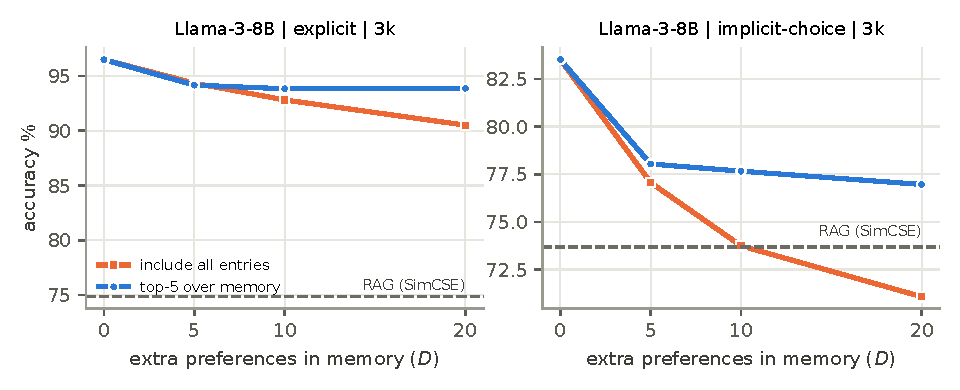
\includegraphics[width=\columnwidth]{p3_stress.pdf}
\caption{Stress test: ``include all'' degrades as the memory grows; top-5 retrieval over the memory levels off.}
\label{fig:stress}
\end{figure}

\subsection{Classifier choice}
Phase~2 compared four detectors and all 15 ensembles: the best ensemble adds only $+0.001$ F1, because the models' errors are highly correlated.
The smallest model (DistilBERT) was therefore sufficient, and it is 51$\times$ faster than LLM-based detection.

%===============================================================================
\section{Discussion}
\begin{itemize}
  \item \textbf{Why memory works.} The failure PrefEval measures is not that the model cannot apply a preference; at 0.2k it applies it about 95\% of
        the time. The failure is that the preference gets lost in the conversation. Restating it next to the question removes the distance between
        the preference and the question that causes the long-context failure.
  \item \textbf{What the classifier contributes.} Deciding what to store is cheap (1.4\,ms per turn) and accurate (98.6--99.9\% of preferences caught,
        almost no false entries). The 14 questions whose preference was missed are answered correctly only 36--50\% of the time at long context, so
        the classifier is the part of the pipeline whose errors matter most.
  \item \textbf{When retrieval is useful.} Retrieval over raw messages is the paper's mechanism, and the new encoder makes it much better. Once a
        memory exists, retrieval is most useful \emph{over the memory}, as the proposal anticipated. This keeps the prompt short when users have many
        preferences.
  \item \textbf{Cost.} At question time the memory adds about \qTokAdd{} prompt tokens (\qTokZs{} $\rightarrow$ \qTokMem). Per turn, it costs one classifier
        pass and one embedding, far cheaper than LLM-based memory writing.
\end{itemize}

%===============================================================================
\section{Limitations}
\begin{itemize}
  \item \textbf{One benchmark with one preference per conversation.} Many-preference behaviour is approximated by a synthetic stress test (one model,
        one length, other-topic preferences only).
  \item \textbf{The classifier is in-distribution.} It was trained on PrefEval-style data from other topics. It catches only 16--26\% of casual
        preferences in real chat (OpenAssistant), so memory recall in the wild would be lower.
  \item \textbf{The strict 5-token metric} penalizes correct but badly formatted answers. It was kept for comparability with the paper.
  \item \textbf{Single deterministic run per cell} (greedy decoding). Differences of 1--2 points between the proposed variants are not claimed as significant;
        the gaps to the baselines (10--35 points) are far larger.
  \item \textbf{Local setup.} Quantized 7--8B models instead of the paper's Bedrock models. The generation task, the implicit-persona form and
        Mistral RAG-Gemma at 10k--23k were not run.
\end{itemize}

%===============================================================================
\section{Conclusion and Future Work}
A cheap trained classifier that writes preferences into a memory, restated before each question, solves most of PrefEval's long-context
preference-following problem for open 7--8B models: \qMiMemTwentyThree\% at 23k tokens versus \qMiRagTwentyThree\% for the paper's best method, at
almost no extra cost. A modern encoder fixes the paper's retrieval bottleneck, but once memory exists, retrieval is best applied over the memory
rather than over raw messages. Future work: evaluate the generation task with a local or API judge; improve real-chat recall of the classifier
with more diverse training data; handle preference updates and conflicts (newer statements overriding older ones); and test on genuinely
multi-preference, multi-session conversations.

\bibliographystyle{IEEEtran}
\bibliography{ref}

%===============================================================================
\appendices
\section{Platforms and Tools}
Experiments ran on a local RTX~3060 workstation, with Ollama (local LLM serving), HuggingFace (models and datasets) and GitHub
(version control). Claude Code (Anthropic) was used as an AI assistant for implementation and writing; the major prompts are listed
in Appendix~B. Code and results: \url{https://github.com/krishnaj01/ML_Project_PrefEval}.

\textbf{Key design decisions.} Local-only evaluation with Ollama; adding Mistral-7B and the long-context regime (Mixtral ruled out after a
feasibility check); four classifiers with ensemble analysis and OpenAssistant data; the strict persona-label filter after a hand-labelled
200-row audit; adding mxbai-embed-large to the encoder comparison; single-message retrieval units; memory entries stored with their context;
the ``Known user preferences'' format; comparison on the full Phase~1 grid; and a multi-preference stress test instead of an oracle-memory bound.

\section{Major Prompts Given to the LLM}
Main instructions, lightly edited for spelling (routine follow-ups and status checks omitted).
\begin{enumerate}
  \item \emph{Setup.} ``This proposal is the SoP for my ML project based on the existing PrefEval paper. Use Ollama for running the model if
        possible, and start from scratch with the environment. I have to run this with a local model, with proper logging, result storing and
        final outputs to compare with the baseline for Phase~1. Tell me which tasks are possible without Amazon Bedrock. Give time estimates
        and tmux commands for long-running tasks, save progressively with a resume option, and tell me when to push to GitHub.''
  \item \emph{Second model.} ``Can we run the same full Phase~1 tiers for Mistral-7B-Instruct-v0.2? Give a proper feasibility analysis, and tell me
        whether Mixtral-8x7B is possible given the system constraints.''
  \item \emph{Phase 2.} ``Let's move on to Phase~2, where I have to train a small classifier. From the four base-model options, give proper
        reasoning and trade-offs so that I can choose the best for our use case, and do real analysis of training and testing: loss curves,
        accuracy, precision/recall, F1, confusion matrix.''
  \item \emph{Audit.} ``When exactly should I put 1 and when 0 in the audit sample, and what if I am unsure? Why is this audit required?''
  \item \emph{Phase 3 plan.} ``Let's plan first: start with the retrieval part, and also add mxbai-embed-large-v1 for comparison, so five
        models in total; then we discuss prompt making and memory. Will embedding the text before the conversation create issues, since it is
        not real-time? How did the paper do it with SimCSE?''
  \item \emph{Memory design.} ``Store the context with each preference. The `Known user preferences' format works. How many preferences should go
        in, since it depends on which preferences occur, where and when: include all, or do RAG over the memory? Should the evaluation be the full
        Phase~1 comparison, or what does the proposal suggest?''
  \item \emph{Final scope.} ``Keep the oracle memory out, but explain exactly what it means first. Include the multi-preference stress test.''
\end{enumerate}

\end{document}
